\documentclass[a4paper,12pt]{article}
\usepackage{amsmath, amssymb, graphicx}

\title{Usos y recomendaciones --- Elementos de transporte y transmisión mecánica}
\author{Joaquín Gómez}
\date{3 de junio, 2025}

\begin{document}
\maketitle

\section*{1. Cálculo de remache con cabeza avellanada (fresada) de diámetro 14 mm}

Para un remache con cabeza fresada, las dimensiones se calculan así:

\[
\begin{aligned}
A &= 1.839 \cdot D = 1.839 \cdot 14\,\text{mm} = 25.746\,\text{mm} \\
C &= 0.5 \cdot D = 0.5 \cdot 14\,\text{mm} = 7\,\text{mm} \\
E &= 0.16 \cdot D = 0.16 \cdot 14\,\text{mm} = 2.24\,\text{mm}
\end{aligned}
\]

\vspace{0.5cm}
\begin{center}
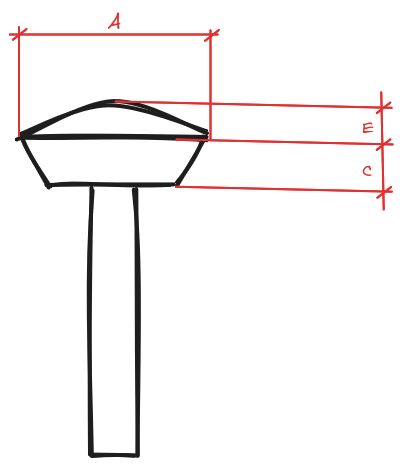
\includegraphics[width=0.4\textwidth]{rosca.png} % Este archivo debe añadirse manualmente
\end{center}

\section*{2. Longitud necesaria de remache con cabeza esférica}

Dado:

\begin{itemize}
\item[$\lambda$] $D = 15\,\text{mm}$
\item[$\lambda$] Espesores: $e = 1.5\,\text{mm}$ (cada cuerpo)
\item[$\lambda$] $n = 2$ cuerpos
\end{itemize}

Fórmula general:

\[
L = l + n \cdot e
\]

\textbf{A mano}:
\[
l = D \cdot 1.5 = 15 \cdot 1.5 = 22.5\,\text{mm}
\Rightarrow L = 22.5 + 2 \cdot 1.5 = 25.5\,\text{mm}
\]

\textbf{A máquina}:
\[
l' = D \cdot 1.7 = 15 \cdot 1.7 = 25.5\,\text{mm}
\Rightarrow L' = 25.5 + 3 = 28.5\,\text{mm}
\]

\section*{3. Tipo de macho y condiciones de trabajo}

\subsection*{Bronce blando (Viruta larga)}

\begin{itemize}
\item[$\lambda$] Machos recomendados: 010, 020, 110, 120 (sin tratamiento)
\item[$\lambda$] Alternativos: 050, 150, 160 (sin tratamiento); 060 (nitrurado); 050 (oxidado al vapor)
\item[$\lambda$] Ángulo de corte: $12^\circ$–$14^\circ$
\item[$\lambda$] Velocidad: $10$–$20\,\text{m/min}$
\item[$\lambda$] Lubricante: Tipo D
\end{itemize}

\subsection*{Baquelita (Viruta corta)}

\begin{itemize}
\item[$\lambda$] Machos recomendados: 010, 020, 110, 120 (nitrurado y con recubrimiento de nitruro de titanio NT)
\item[$\lambda$] Ángulo de corte: $3^\circ$–$5^\circ$
\item[$\lambda$] Velocidad: $6$–$12\,\text{m/min}$
\item[$\lambda$] Lubricante: Tipo F
\end{itemize}

\section*{4. Identificación de material de macho}

Macho alternativo con:

\begin{itemize}
\item[$\lambda$] Tratamiento superficial: Nitrurado + Nitruro de Titanio (NT)
\item[$\lambda$] Viruta: Corta y larga (C/L)
\item[$\lambda$] Ángulo de corte: $10^\circ$–$12^\circ$
\item[$\lambda$] Lubricante: B–E (1)(3)(4)
\end{itemize}

\textbf{Material correspondiente: Fundición esferoidal}

\section*{5. Significado de numeración 4.6 en tornillos}

Norma ISO:

\[
\text{Resistencia a la tracción: } 4 \cdot 100 = 400\,\text{MPa}
\]
\[
\text{Límite elástico: } 400 \cdot \frac{6}{10} = 240\,\text{MPa}
\]

\textbf{Aplicación}: Tornillos de baja carga estructural.

\section*{6. Cálculo de fuerza en un momento torsor}

Datos:
\[
M = 30\,\text{Nm},\quad d = 20\,\text{cm} = 0.2\,\text{m}
\]
\[
F = \frac{M}{d} = \frac{30}{0.2} = 150\,\text{N}
\]

\section*{7. Profundidad de rosca}

\[
\text{Paso normal: } P = 2\,\text{mm},\quad h = 0.7 \cdot P = 1.4\,\text{mm}
\]
\[
\text{Paso fino: } P = 1.5\,\text{mm},\quad h = 0.7 \cdot 1.5 = 1.05\,\text{mm}
\]

\section*{8. Diámetro de varilla roscada (rosca Whitworth)}

\begin{itemize}
\item[$\lambda$] Diámetro nominal: $D = \frac{3}{16} = 4.76\,\text{mm}$
\item[$\lambda$] Paso: $P = \frac{1}{24} = 1.06\,\text{mm}$
\item[$\lambda$] Diámetro efectivo:
\[
d = D - 0.1 \cdot P = 4.76 - 0.1 \cdot 1.06 = 4.65\,\text{mm}
\]
\end{itemize}

\textbf{Tipo de rosca:} Whitworth

\section{Ejercicios 2}

\begin{enumerate}
    \item Reconocer cual es el trabajo realizado con un macho que tiene un tipo de agujero 1 en una fundición maleable.
           \begin{itemize}
            \item[$\lambda$] Recomendados: 050 (nitrurado)
            \item[$\lambda$] Alternativos: 060 (nitrurado y nitrurado titano, NT)
            \item[$\lambda$] Velocidad: $6 \,-\, 12 m/min$
            \item[$\lambda$] Ángulo de corte: $7^{\circ} \, - \, 9^{\circ}$
            \item[$\lambda$] Lubricante: $B-E(1)(3)(4)$
        \end{itemize}
            
            

\end{enumerate}

\end{document}
